\documentclass[12pt, a4paper, oneside]{ctexart}
\usepackage{amsmath, amsthm, amssymb, bm, color, graphicx, geometry, mathrsfs,extarrows, braket, booktabs, array, xcolor, fontspec, appendix, float, subfigure, wrapfig, enumitem, titlesec}
\usepackage[colorlinks,linkcolor=red,anchorcolor=blue,citecolor=blue,urlcolor=blue,menucolor=black]{hyperref}
\usepackage{tabularx}

%%%% 设置中文字体 %%%%
% fc-list -f "%{family}\n" :lang=zh >d:zhfont.txt 命令查看已有字体
\setCJKmainfont[
    BoldFont=方正黑体_GBK,  % 黑体
    ItalicFont=方正楷体_GBK,  % 楷体
    BoldItalicFont=方正粗楷简体,  % 粗楷体
    Mapping = fullwidth-stop  % 将中文句号“.”全部转化为英文句号“.”,
]{方正书宋简体}  % !!! 注意在Windows中运行请改为“方正书宋简体.ttf” !!!
%%%% 设置英文字体 %%%%
\setmainfont{Minion Pro}
\setsansfont{Calibri}
\setmonofont{Consolas}

%%%% 设置代码块 %%%%
% 在vscode中使用minted需要先配置python解释器, Ctrl+Shift+P, 输入Python: Select Interpreter选择安装了Pygments的Python版本. 再在setting.json中xelatex和pdflatex的参数中加入 "--shell-escape", 即可
% TeXworks中配置方法参考: https://blog.csdn.net/RobertChenGuangzhi/article/details/108140093
\usepackage{minted}
\renewcommand{\theFancyVerbLine}{
    \sffamily\textcolor[rgb]{0.5,0.5,0.5}{\scriptsize\arabic{FancyVerbLine}}} % 修改代码前序号大小
% 加入不同语言的代码块
\newmintinline{cpp}{fontsize=\small, linenos, breaklines, frame=lines}
\newminted{cpp}{fontsize=\small, baselinestretch=1, linenos, breaklines, frame=lines}
\newmintedfile{cpp}{fontsize=\small, baselinestretch=1, linenos, breaklines, frame=lines}
\newmintinline{matlab}{fontsize=\small, linenos, breaklines, frame=lines}
\newminted{matlab}{fontsize=\small, baselinestretch=1, mathescape, linenos, breaklines, frame=lines}
\newmintedfile{matlab}{fontsize=\small, baselinestretch=1, linenos, breaklines, frame=lines}
\newmintinline{python}{fontsize=\small, linenos, breaklines, frame=lines, python3}  % 使用\pythoninline{代码}
\newminted{python}{fontsize=\small, baselinestretch=1, linenos, breaklines, frame=lines, python3}  % 使用\begin{pythoncode}代码\end{pythoncode}
\newmintedfile{python}{fontsize=\small, baselinestretch=1, linenos, breaklines, frame=lines, python3}  % 使用\pythonfile{代码地址}

%%%% 设置行间距与页边距 %%%%
\linespread{1.2}
\geometry{left=2.5cm, right=2.5cm, top=2.5cm, bottom=2.5cm}
% \geometry{left=1.84cm,right=1.84cm,top=2.18cm,bottom=2.18cm}  % 更小的页边距

%%%% 定理类环境的定义 %%%%
\newtheorem{example}{例}            % 整体编号
\newtheorem{theorem}{定理}[section] % 定理按section编号
\newtheorem{definition}{定义}
\newtheorem{axiom}{公理}
\newtheorem{property}{性质}
\newtheorem{proposition}{命题}
\newtheorem{lemma}{引理}
\newtheorem{corollary}{推论}
\newtheorem{condition}{条件}
\newtheorem{conclusion}{结论}
\newtheorem{assumption}{假设}
\numberwithin{equation}{section}  % 公式按section编号 (公式右端的小括号)
\newtheorem{algorithm}{算法}

%%%% 自定义环境 %%%%
\newsavebox{\nameinfo}
\newenvironment{myTitle}[1]{
    \begin{center}
    {\zihao{-2}\bf #1\\}
    \zihao{-4}\it
}{\end{center}}  % \begin{myTitle}{标题内容}作者信息\end{myTitle}
\newcounter{problem}  % 问题序号计数器
\newenvironment{problem}[1][]{\stepcounter{problem}\par\noindent\textbf{题目\arabic{problem}. #1}}{\smallskip\par}
\newenvironment{solution}[1][]{\par\noindent\textbf{#1解答. }}{\smallskip\par}  % 可带一个参数表示题号\begin{solution}{题号}
\newenvironment{note}{\par\noindent\textbf{注记. }}{\smallskip\par}
\newenvironment{remark}{\begin{enumerate}[label=\textbf{注\arabic*.}]}{\end{enumerate}}
\BeforeBeginEnvironment{minted}{\vspace{-0.5cm}}  % 缩小minted环境距上文间距
\AfterEndEnvironment{minted}{\vspace{-0.2cm}}  % 缩小minted环境距下文间距

%%%% 自定义段落开头序号,间距 (titlesec) %%%%
% 中文序号:\zhnum{section}, 阿拉伯序号:\arabic
\titleformat{\section}{\Large\bfseries}{\arabic{section}}{1em}{}[]
\titlespacing{\section}{0pt}{1.2ex plus .0ex minus .0ex}{.6ex plus .0ex}
\titlespacing{\subsection}{0pt}{1.2ex plus .0ex minus .0ex}{.6ex plus .0ex}
\titlespacing{\subsubsection}{0pt}{1.2ex plus .0ex minus .0ex}{.6ex plus .0ex}

%%%% 图片相对路径 %%%%
\graphicspath{{figures/}} % 当前目录下的figures文件夹, {../figures/}则是父目录的figures文件夹
\setlength{\abovecaptionskip}{-0.2cm}  % 缩紧图片标题与图片之间的距离
\setlength{\belowcaptionskip}{0pt} 

%%%% 缩小item,enumerate,description两行间间距 %%%%
\setenumerate[1]{itemsep=0pt,partopsep=0pt,parsep=\parskip,topsep=5pt}
\setitemize[1]{itemsep=0pt,partopsep=0pt,parsep=\parskip,topsep=5pt}
\setdescription{itemsep=0pt,partopsep=0pt,parsep=\parskip,topsep=5pt}

%%%% 自定义公式 %%%%
\everymath{\displaystyle} % 默认全部行间公式, 想要变回行内公式使用\textstyle
\DeclareMathOperator*\uplim{\overline{lim}}     % 定义上极限 \uplim_{}
\DeclareMathOperator*\lowlim{\underline{lim}}   % 定义下极限 \lowlim_{}
\DeclareMathOperator*{\argmax}{arg\,max}  % 定义取最大值的参数 \argmax_{}
\DeclareMathOperator*{\argmin}{arg\,min}  % 定义取最小值的参数 \argmin_{}
\let\leq=\leqslant % 简写小于等于\leq (将全部leq变为leqslant)
\let\geq=\geqslant % 简写大于等于\geq (将全部geq变为geqslant)
\DeclareRobustCommand{\rchi}{{\mathpalette\irchi\relax}}
\newcommand{\irchi}[2]{\raisebox{\depth}{$#1\chi$}} % 使用\rchi将\chi居中

%%%% 一些宏定义 %%%%
\def\bd{\boldsymbol}        % 加粗(向量) boldsymbol
\def\disp{\displaystyle}    % 使用行间公式 displaystyle(默认)
\def\tsty{\textstyle}       % 使用行内公式 textstyle
\def\sign{\text{sign}}      % sign function
\def\wtd{\widetilde}        % 宽波浪线 widetilde
\def\R{\mathbb{R}}          % Real number
\def\N{\mathbb{N}}          % Natural number
\def\Z{\mathbb{Z}}          % Integer number
\def\Q{\mathbb{Q}}          % Rational number
\def\C{\mathbb{C}}          % Complex number
\def\K{\mathbb{K}}          % Number Field
\def\P{\mathbb{P}}          % Polynomial
\def\E{\mathbb{E}}          % Exception
\def\d{\mathrm{d}}          % differential operator
\def\e{\mathrm{e}}          % Euler's number
\def\i{\mathrm{i}}          % imaginary number
\def\re{\mathrm{Re}}        % Real part
\def\im{\mathrm{Im}}        % Imaginary part
\def\res{\mathrm{Res}}      % Residue
\def\ker{\mathrm{Ker}}      % Kernel
\def\vspan{\mathrm{vspan}}  % Span  \span与latex内核代码冲突改为\vspan
\def\L{\mathcal{L}}         % Loss function
\def\O{\mathcal{O}}         % big O notation
\def\wdh{\widehat}          % 宽帽子 widehat
\def\ol{\overline}          % 上横线 overline
\def\ul{\underline}         % 下横线 underline
\def\add{\vspace{1ex}}      % 增加行间距
\def\del{\vspace{-1.5ex}}   % 减少行间距

%%%% 正文开始 %%%%
\begin{document}

%%%% 定义标题页,包括title,author,affiliation,email等 %%%%
\title{嵌入式智能计算系统\\读书报告}
\author{
西安交通大学, 人工智能学院, B2480 \\[10ex]
吴天阳\\[1ex]
4124136039\\[1ex]
tianyang-wu@stu.xjtu.edu.cn\\[2ex]
}
\date{\today}
\pagenumbering{gobble} % 暂时关闭页码
\maketitle % 设置上面的标题
\clearpage % 创建新的一面
\tableofcontents % 创建目录页,使用目录需要编译两次, 并且不能删去编译产生的临时文件!!!

%%%% 以下部分是正文 %%%%  
\clearpage
\section{类脑计算的概念}
类脑计算,又称神经形态计算(Neuromorphic Computing),
是一种受到生物神经系统信息处理模式和结构启发的计算范式。
它旨在模仿人脑神经网络的结构和功能,从而实现更高效、更低功耗的计算。
类脑计算并非简单地复制人脑,而是借鉴人脑的认知机理,
建立一种不同于传统冯·诺依曼架构的、受脑启发的计算模式\cite{ref1}。
\begin{figure}[htbp]
    \centering
    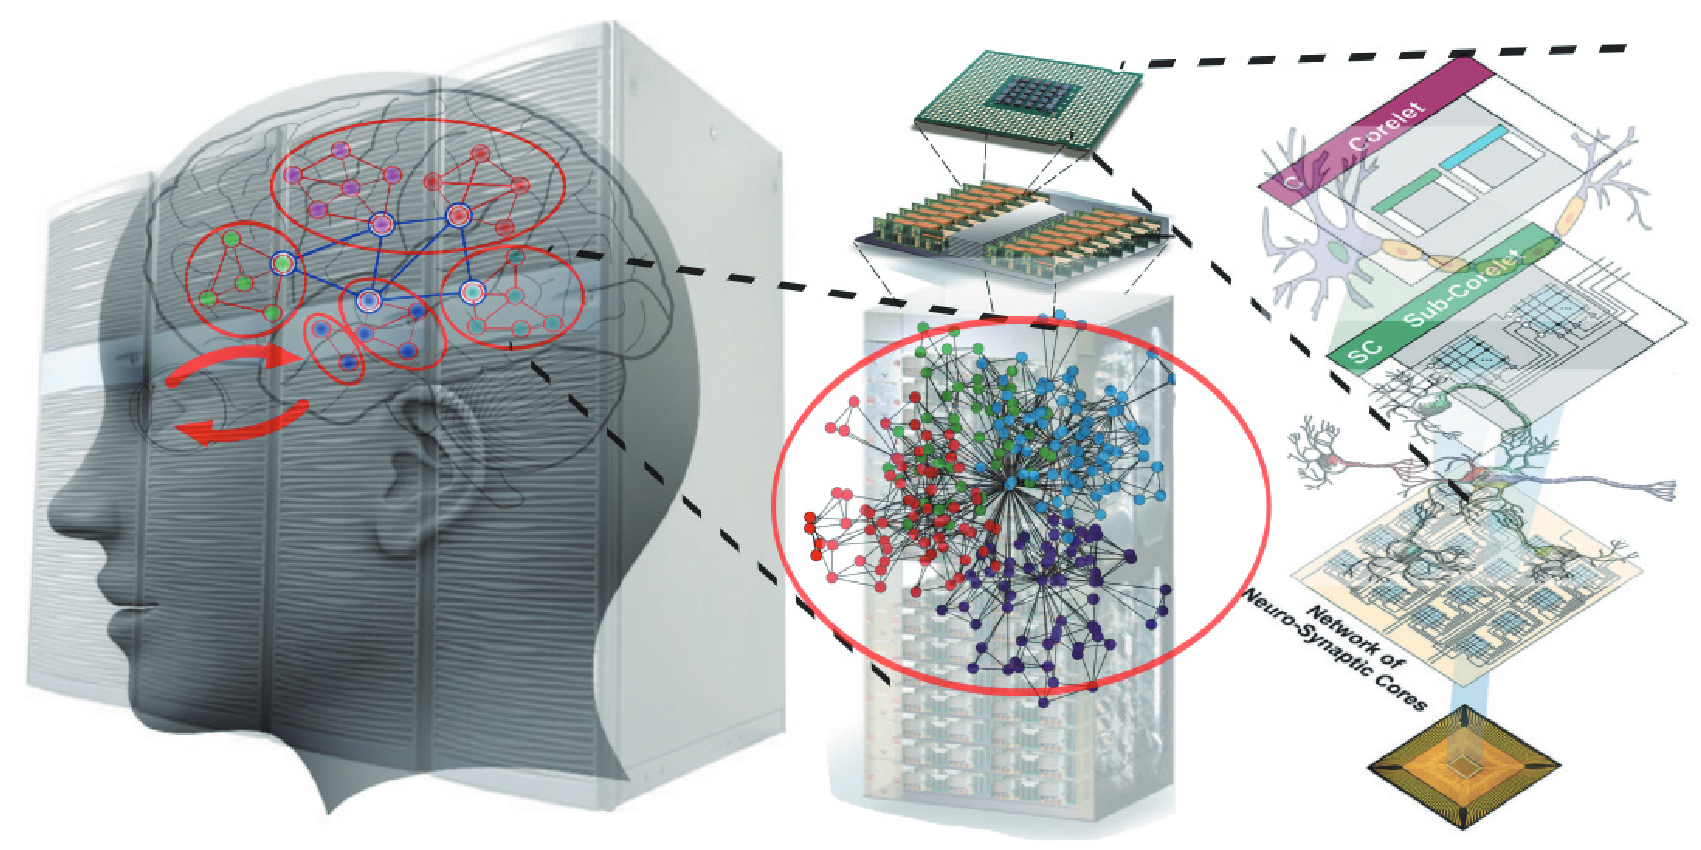
\includegraphics[width=\linewidth]{1.png}
    \caption{类脑计算的一种基本架构}
\end{figure}

\paragraph{核心思想}
\begin{itemize}
    \item 模仿生物神经系统:类脑计算的核心在于模拟生物神经网络的结构和信息加工过程,
    例如神经元、突触以及脉冲信号等。
    \item 非冯·诺依曼架构:传统计算机采用冯·诺依曼架构,将存储器和处理器分离,
    数据需要在两者之间频繁传输,造成“存储墙”瓶颈。类脑计算则借鉴人脑存算一体的特点,旨在突破这一瓶颈。
    \item 高效低功耗: 人脑在处理复杂信息时展现出惊人的效率和极低的功耗。
    类脑计算希望能够模拟人脑的这些优势,实现更高效、更节能的计算。
\end{itemize}

\paragraph{类脑计算的意义}
\begin{itemize}
    \item 突破传统计算瓶颈: 随着数据量的爆炸式增长和计算任务的日益复杂,传统冯·诺依曼架构的计算能力面临挑战。
    类脑计算有望突破传统架构的限制,提供更强大的计算能力。
    \item 发展新一代人工智能: 类脑计算被认为是实现通用人工智能的重要途径之一。
    通过模拟人脑的工作方式,有望在感知、认知、学习等方面取得突破。
    \item 推动神经科学研究: 类脑计算的研究也能够反过来促进神经科学的发展,
    帮助人们更深入地理解人脑的工作原理。
\end{itemize}

总而言之,类脑计算是一种革命性的计算范式,它从生物神经系统中汲取灵感,
旨在构建更智能、更高效、更节能的计算系统,为人工智能的未来发展开辟新的道路。

\section{脉冲神经元模型}
脉冲神经元模型是脉冲神经网络(SNN)的基本组成单元,
它模拟生物神经元的电生理特性和信息处理方式。
与传统神经网络中使用的sigmoid或ReLU神经元模型不同,
脉冲神经元模型以脉冲(spike)作为信息传递和处理的基本单元,
更接近生物神经元的真实工作方式\cite{ref2,ref3}。
\begin{figure}[htbp]
    \centering
    
\includegraphics[width=\linewidth]{2.png}
    \caption{SRNN结构图}
\end{figure}

\subsection{常见的脉冲神经元模型}
\begin{itemize}
    \item Hodgkin-Huxley 模型 (HH模型): HH模型是最经典的生物神经元模型之一,
    它通过一组非线性微分方程精确地描述了神经元膜电位的动态变化过程,
    包括离子通道的开放和关闭、动作电位的产生和传播等。HH模型生物学真实性高,
    但计算复杂度也较高。
    \item Leaky Integrate-and-Fire 模型 (LIF模型): LIF模型是对HH模型的简化,
    它在保持生物合理性的同时,大大降低了计算复杂度,
    成为SNN中最常用的神经元模型之一。LIF模型将神经元的膜电位视为一个电容器的电压,
    当接收到来自其他神经元的电流输入时,电容器充电;同时,
    电容器会以一定的速率自行放电(leaky)。当膜电位超过阈值时,
    神经元产生一个脉冲(fire),然后膜电位被重置。

    LIF模型的基本公式:
    \begin{equation}
        \tau_m * \d V_m/dt = -(V_m - V_{rest}) + R_m * I_e(t)
    \end{equation}
    其中$V_m$为膜电位,$\tau_m$为膜时间常数,$V_rest$为静息电位,
    $R_m$为膜电阻,$I_e(t)$为外部输入电流。
    \item 其他脉冲神经元模型:  除了HH模型和LIF模型,还有其他一些脉冲神经元模型,例如:
    \begin{itemize}
        \item Izhikevich 模型: 在计算复杂度和生物合理性之间取得了较好的平衡。
        \item Integrate-and-Fire 模型 (IF模型): LIF模型的更简化版本,忽略了膜的泄漏特性。
        \item Quadratic Integrate-and-Fire 模型 (QIF模型): 在阈值附近具有二次电压依赖性的模型。
    \end{itemize}
\end{itemize}

\subsection{脉冲神经元模型的特点}
\begin{itemize}
    \item 事件驱动: 脉冲神经元只有在接收到足够强度的输入时才会发放脉冲,这种事件驱动的特性使得SNN具有更高的计算效率和更低的功耗。
    \item 时间编码: 脉冲神经元模型能够处理时间信息,例如脉冲发放的时间、频率和模式等,这使得SNN更适合处理时序数据,如语音、视频等。
    \item 非线性动力学: 脉冲神经元模型具有复杂的非线性动力学特性,能够模拟生物神经元的多种放电模式,例如规则放电、簇状放电、混沌放电等。
\end{itemize}

脉冲神经元模型是SNN的核心,选择合适的神经元模型对于构建高性能的SNN至关重要。不同的神经元模型在生物合理性、计算复杂度和适用场景等方面各有优缺点,需要根据具体的应用需求进行选择。

\section{脉冲神经网络 SNN}
脉冲神经网络(Spiking Neural Networks, SNNs)是第三代神经网络,它以脉冲神经元模型为基础构建,更真实地模拟了生物神经网络的信息处理方式。SNNs 不仅考虑神经元的激活状态,还强调脉冲发放的时间和频率,通过脉冲序列进行信息编码和传递。
\begin{figure}[htbp]
    \centering
    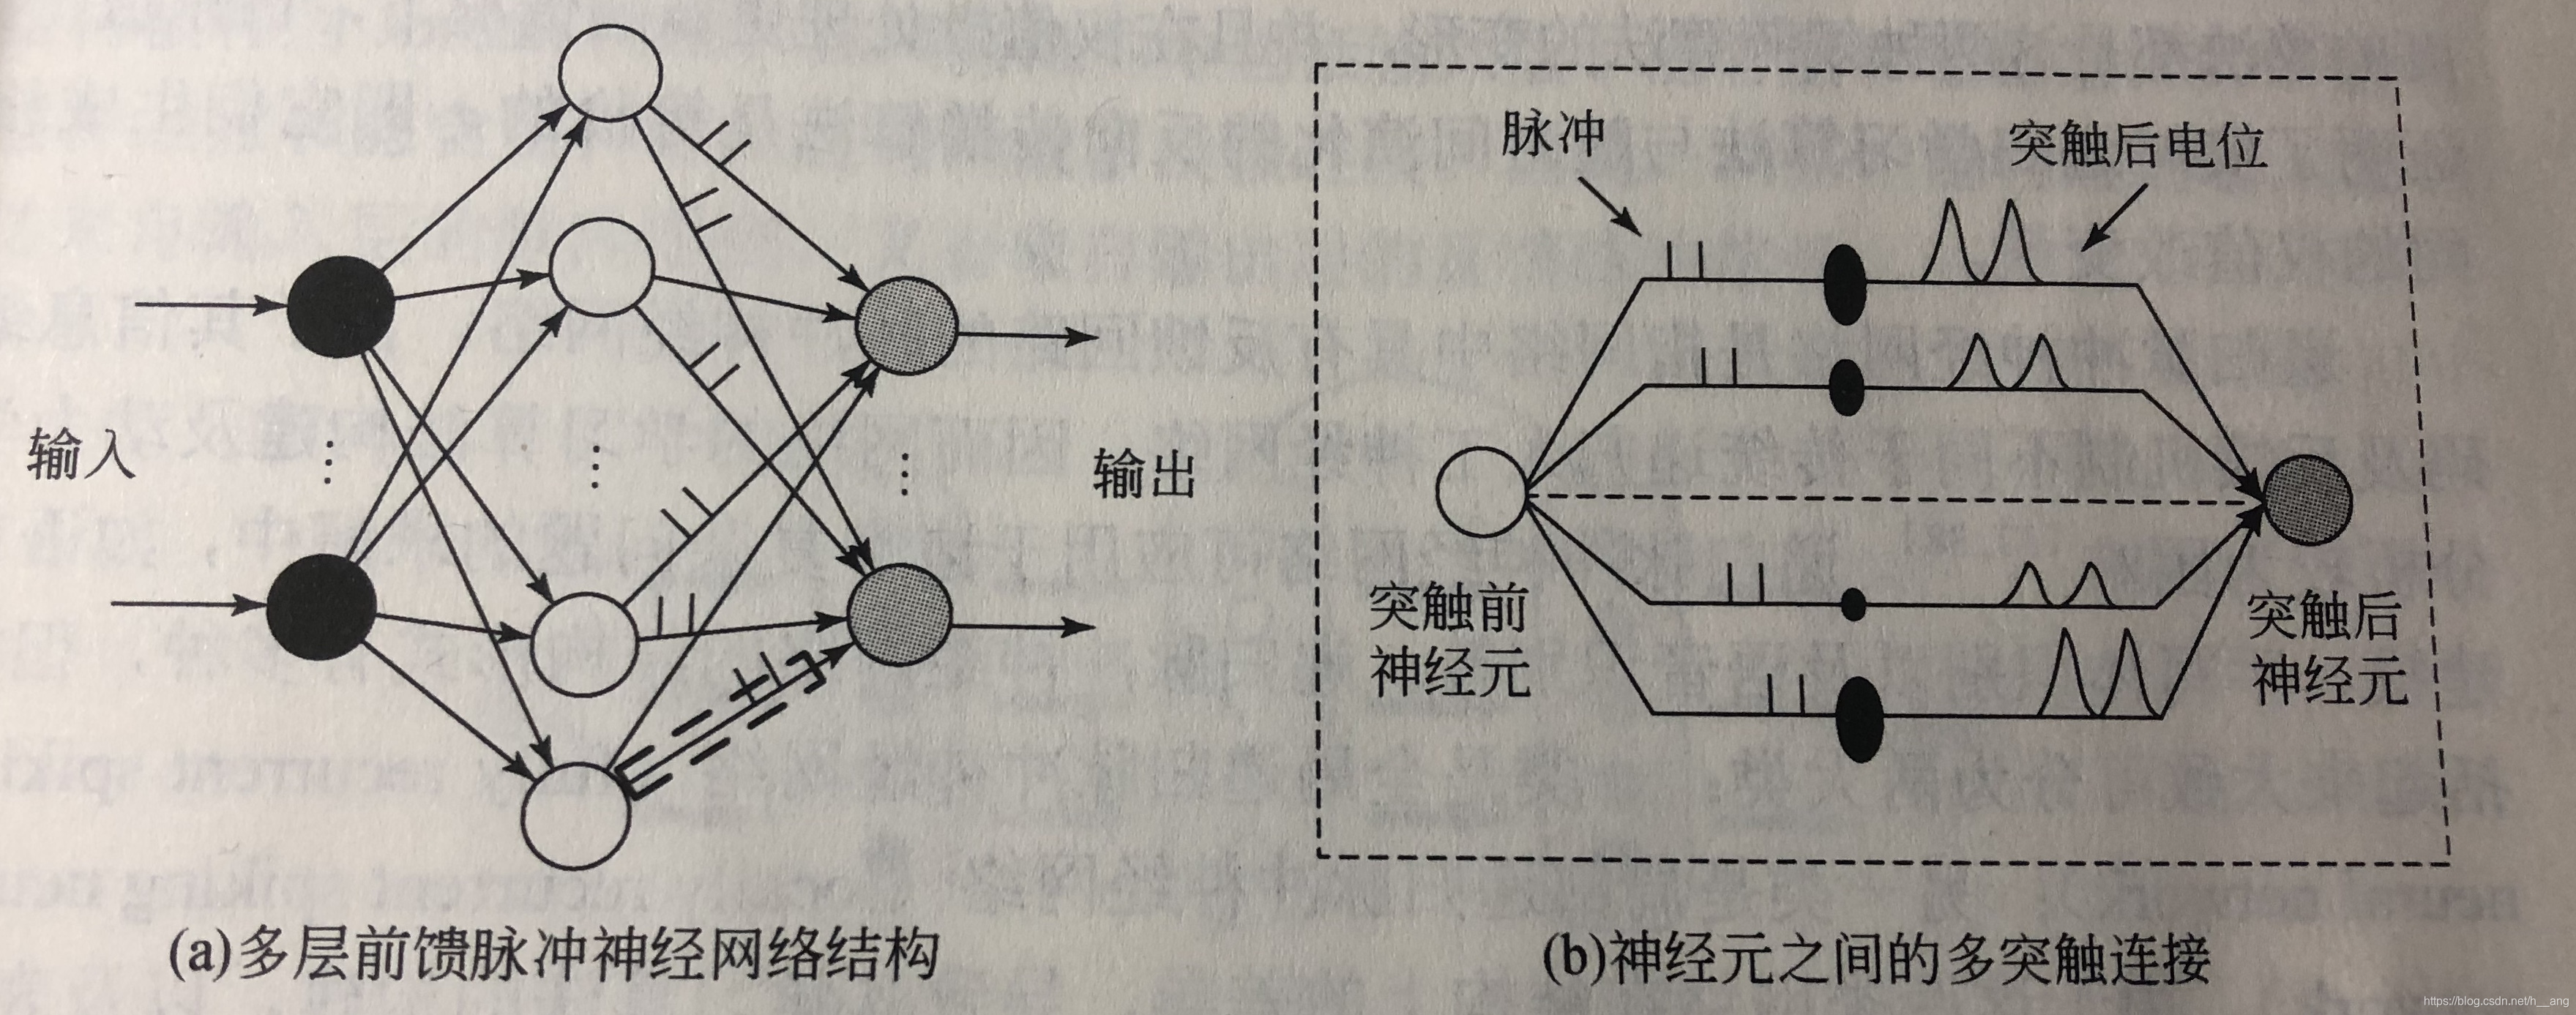
\includegraphics[width=\linewidth]{3.jpeg}
    \caption{前馈型脉冲神经网络}
\end{figure}
\subsection{SNN 的基本结构}
SNN 的基本结构与传统神经网络类似,通常包括:
\begin{itemize}
    \item 输入层: 负责接收外部输入信号,并将输入信号转换为脉冲序列。
    \item 隐藏层: 由脉冲神经元相互连接构成,负责进行信息处理和特征提取。SNN 可以包含单层或多层隐藏层。
    \item 输出层: 将隐藏层的脉冲信号解码为最终的输出结果。
\end{itemize}
\subsection{SNN 的信息编码方式}
SNN 使用多种脉冲编码方式来表示信息,常见的包括:
\begin{itemize}
    \item 率编码 (Rate Coding): 信息编码在脉冲发放的频率上。较高的脉冲频率代表较高的输入强度或特征值。率编码是 SNN 中最常用的编码方式之一。
    \item 时间编码 (Temporal Coding): 信息编码在脉冲发放的时间上。例如,延迟编码 (latency coding) 使用首个脉冲发放的时间来编码信息;时间差编码 (spike-time difference coding) 使用不同神经元脉冲发放时间差来编码信息。时间编码能够更有效地利用时间信息,具有更高的信息容量和更快的响应速度。
    \item 群体编码 (Population Coding): 信息编码在神经元群体的脉冲发放模式上。通过多个神经元协同工作,共同表示和处理信息,提高 SNN 的鲁棒性和容错性。
\end{itemize}
\subsection{SNN 的学习机制}
SNN 的学习机制是研究的热点和难点。与传统神经网络的反向传播算法 (Backpropagation, BP) 不同,SNN 通常采用生物 plausibility 更高的学习算法,例如:
\begin{itemize}
    \item 脉冲时序依赖可塑性 (Spike-Timing Dependent Plasticity, STDP):  STDP 是一种基于突触前后脉冲发放时序的局部学习规则。当突触前脉冲早于突触后脉冲到达时,突触连接强度增强 (LTP, Long-Term Potentiation);反之,当突触前脉冲晚于突触后脉冲到达时,突触连接强度减弱 (LTD, Long-Term Depression)。STDP 能够有效地学习时序信息和因果关系。
    \item 其他学习算法:  除了 STDP,还有其他一些 SNN 学习算法,例如:
    \begin{itemize}
        \item 监督学习算法: 将 BP 算法 modified 后应用于 SNN,例如 SpikeProp, BP-SNN 等。
        \item 无监督学习算法: 基于 STDP 的变体,例如 MSTDP, Reward-modulated STDP 等。
        \item 强化学习算法: 将强化学习与 SNN 结合,例如 Spiking Actor-Critic, Deep Spiking Q-Network 等。
    \end{itemize}
\end{itemize}
\subsection{SNN 的特点}
\begin{itemize}
    \item 生物合理性: SNN 更接近生物神经网络的真实工作方式,为神经科学研究提供了有力的工具。
    \item 低功耗: SNN 的事件驱动特性和脉冲信号的稀疏性,使其在功耗方面具有显著优势,尤其适合于低功耗应用场景,如移动设备、物联网设备等。
    \item 时序信息处理能力: SNN 能够自然地处理时序信息,例如语音、视频、时间序列预测等,在时序数据处理领域具有优势。
    \item 硬件友好性: SNN 的脉冲信号和事件驱动特性,使其更易于在新型神经形态硬件上实现高效运行。
\end{itemize}

然而,SNN 的研究和应用仍然面临一些挑战,例如:
\begin{itemize}
    \item 学习算法的复杂性: SNN 的学习算法相对 ANN 更加复杂,训练 SNN 模型通常需要更多的时间和计算资源。
    \item 模型优化的难度: SNN 的模型参数众多,优化难度较大,需要更有效的模型优化方法。
    \item 硬件实现的挑战: 虽然 SNN 与神经形态硬件天然契合,但大规模、高性能 SNN 硬件的实现仍然面临技术挑战。
\end{itemize}

尽管如此,SNN 作为一种新兴的神经网络模型,凭借其独特的优势,在人工智能领域展现出巨大的潜力,尤其是在低功耗智能、时序数据处理、神经科学研究等方向具有广阔的应用前景。
\section{SNN 与其他类型神经网络对比}
脉冲神经网络 (SNN) 与其他类型的神经网络,如人工神经网络 (ANN) 和循环神经网络 (RNN),在模型结构、信息编码、计算方式、应用场景等方面存在显著差异\cite{ref4,ref5}。
\subsection{与人工神经网络 (ANN) 的对比}
\begin{figure}[H]
  \centering
  \subfigure{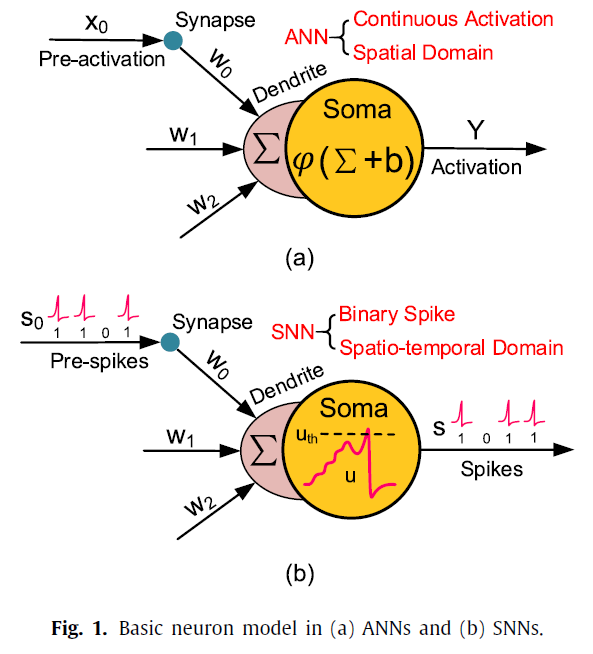
\includegraphics[width=0.49\textwidth]{4.1.png}}
  \subfigure{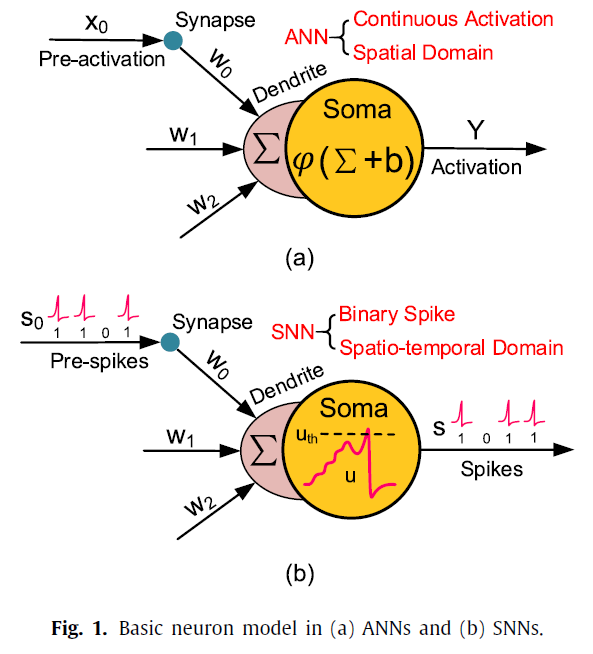
\includegraphics[width=0.49\textwidth]{4.2.png}}
  \setlength{\abovecaptionskip}{0ex}  % 如果使用了minted会增大图像与标题间距需要进行缩小
  \label{fig-snn-ann}
  \caption{SNN与ANN比较图}
\end{figure}
\begin{table}[!h]
\caption{SNN与ANN比较} \label{tabel-snn-ann} \vspace{2mm}
\begin{tabularx}{\textwidth}{lll}
\toprule
\multicolumn{1}{c}{\textbf{特性}} & \multicolumn{1}{c}{\textbf{人工神经网络 (ANN)}} & \multicolumn{1}{c}{\textbf{脉冲神经网络 (SNN)}}                           \\ \midrule
\textbf{神经元模型}                  & Sigmoid, ReLU 等连续激活函数                     & 脉冲神经元模型 (LIF, HH 等)                                                 \\
\textbf{信息编码}                   & 连续值                                       & 脉冲序列 (离散事件)                                                         \\
\textbf{计算方式}                   & 连续值运算 (乘法累加)                              & 事件驱动计算 (加法为主)                                                       \\
\textbf{时间特性}                   & 静态模型,不显式处理时间信息                            & 动态模型,显式处理时间信息                                                       \\
\textbf{功耗}                     & 相对较高                                      & 相对较低                                                                \\
\textbf{生物合理性}                  & 较低                                        & 较高                                                                  \\
\textbf{应用场景}                   & 图像识别、自然语言处理等成熟领域                          & \begin{tabular}[c]{@{}l@{}}低功耗应用、时序数据处理、\\ 神经科学研究等新兴领域\end{tabular} \\
\textbf{学习算法}                   & 反向传播算法 (BP)                               & \begin{tabular}[c]{@{}l@{}}STDP, BP 改进算法, \\ 其他生物启发算法\end{tabular}  \\
\textbf{硬件实现}                   & GPU, ASIC 等加速器                            & 神经形态芯片                                                              \\
\textbf{发展阶段}                   & 成熟,应用广泛                                   & 发展中,潜力巨大                                                            \\ \bottomrule
\end{tabularx}
\end{table}
如表\ref{tabel-snn-ann}所示,二者主要差异总结如下:
\begin{itemize}
    \item 信息表示和计算: ANN 使用连续值进行信息表示和计算,计算方式以乘法累加为主;SNN 使用脉冲序列进行信息表示,计算方式以事件驱动的加法为主。SNN 的脉冲计算更加稀疏和节能。
    \item 时间特性: ANN 通常是静态模型,不显式处理时间信息;SNN 是动态模型,能够自然地处理时间信息,更适合处理时序数据。
    \item 功耗: 由于事件驱动和脉冲稀疏性,SNN 在理论上具有更低的功耗。
    \item 生物合理性: SNN 更接近生物神经网络的工作方式,生物合理性更高,有助于神经科学研究。
    \item 应用领域: ANN 在图像识别、自然语言处理等领域取得了巨大成功,应用成熟;SNN 在低功耗应用、时序数据处理、神经科学研究等新兴领域展现出潜力。
\end{itemize}
\subsection{与循环神经网络 (RNN) 的对比}
RNN 也是一种能够处理时序信息的神经网络,但与 SNN 相比,仍然存在显著差异,如表\ref{tabel-snn-rnn}所示:
\begin{table}[!h]
\caption{SNN与RNN比较} \label{tabel-snn-rnn} \vspace{2mm}
\begin{tabularx}{\textwidth}{lll}
\toprule
\multicolumn{1}{c}{\textbf{特性}} & \multicolumn{1}{c}{\textbf{循环神经网络 (RNN)}} & \multicolumn{1}{c}{\textbf{脉冲神经网络 (SNN)}}                        \\ \midrule
\textbf{神经元模型}                  & Sigmoid, ReLU 等连续激活函数                     & 脉冲神经元模型 (LIF, HH 等)                                              \\
\textbf{信息编码}                   & 连续值                                       & 脉冲序列 (离散事件)                                                      \\
\textbf{时间处理}                   & 通过循环连接处理时序信息                              & \begin{tabular}[c]{@{}l@{}}通过神经元动力学和脉冲时序\\ 自然处理时序信息\end{tabular} \\
\textbf{计算方式}                   & 连续值运算 (乘法累加)                              & 事件驱动计算 (加法为主)                                                    \\
\textbf{功耗}                     & 相对较高 (相比 SNN)                             & 相对较低                                                             \\
\textbf{生物合理性}                  & 较低 (相比 SNN)                               & 较高                                                               \\
\textbf{擅长领域}                   & 自然语言处理、序列预测等                              & \begin{tabular}[c]{@{}l@{}}低功耗时序数据处理、\\ 神经科学研究等\end{tabular}     \\
\textbf{梯度消失/爆炸}                & 存在                                        & 缓解 (脉冲事件驱动)                                                      \\ \bottomrule
\end{tabularx}
\end{table}

差异总结:
\begin{itemize}
    \item 时间处理机制: RNN 通过循环连接来处理时序信息,本质上仍然是离散时间模型;SNN 通过神经元动力学和脉冲时序自然地处理时间信息,是连续时间模型,更符合生物神经系统的工作方式。
    \item 梯度问题: RNN 在处理长时序数据时容易出现梯度消失或梯度爆炸问题;SNN 的事件驱动特性在一定程度上缓解了梯度问题。
    \item 功耗和生物合理性: SNN 在功耗和生物合理性方面优于 RNN。
\end{itemize}
\subsection{总结}
SNN 作为第三代神经网络,与 ANN 和 RNN 等传统神经网络相比,在信息表示、计算方式、时间特性、功耗和生物合理性等方面都展现出独特的优势。虽然 SNN 的发展仍面临挑战,但其在低功耗智能、时序数据处理和神经科学研究等领域具有广阔的应用前景,是未来神经网络发展的重要方向之一。

\section{类脑芯片如何支持 SNN 计算}
类脑芯片,也称为神经形态芯片,是一种专门为运行脉冲神经网络 (SNN) 而设计的新型计算硬件。与传统的冯·诺依曼架构芯片不同,类脑芯片借鉴了生物大脑的结构和工作原理,旨在实现更高效、更低功耗的 SNN 计算\cite{ref6,ref7,ref8}。

\subsection{类脑芯片支持 SNN 计算的关键特性}
\begin{itemize}
    \item 神经元和突触的硬件实现: 类脑芯片的核心在于使用硬件电路直接模拟脉冲神经元和突触的功能。
    \begin{itemize}
        \item 神经元电路: 使用模拟或数字电路实现脉冲神经元模型 (如 LIF, HH 等) 的膜电位动态、脉冲发放和重置等行为。模拟电路能够更精确地模拟生物神经元的特性,但可编程性较差;数字电路则具有更高的灵活性和可扩展性。混合信号电路 (数模混合) 结合了模拟电路和数字电路的优点,成为一种重要的发展方向。
        \item 突触电路: 实现突触的连接强度 (权重) 和可塑性。忆阻器 (memristor) 等新型纳米器件由于其类突触特性 (电阻可调、非易失性等),被认为是构建高效突触电路的理想选择。
    \end{itemize}
    \item 事件驱动架构:  类脑芯片采用事件驱动的异步计算架构,只在脉冲事件发生时才进行计算,避免了传统同步计算架构中大量无效计算,显著降低了功耗。
    \item 并行分布式计算:  类脑芯片通常采用大规模并行分布式架构,将大量的神经元和突触单元集成在芯片上,实现高效的并行计算,加速 SNN 的运行速度。
    \item 片上学习能力:  为了充分发挥 SNN 的潜力,类脑芯片需要支持片上学习功能,即在芯片本地进行模型训练和参数更新。这需要硬件实现各种 SNN 学习算法 (如 STDP) 以及相应的参数存储和更新机制。
    \item 低功耗设计:  低功耗是类脑芯片的重要优势之一。通过采用事件驱动架构、模拟/混合信号电路、新型低功耗器件等技术,类脑芯片能够实现远低于传统芯片的功耗水平。
\end{itemize}
\subsection{类脑芯片支持 SNN 计算的方式}
\begin{itemize}
    \item 硬件加速 SNN 运算: 类脑芯片通过硬件电路直接实现神经元和突触的功能,能够并行高效地执行 SNN 的运算,加速 SNN 的推理和训练过程。
    \item 降低功耗: 事件驱动架构和脉冲计算的稀疏性使得类脑芯片在运行 SNN 时具有极低的功耗,尤其适合于边缘计算和移动设备等功耗敏感的应用场景。
    \item 支持生物学习算法: 类脑芯片可以硬件实现各种生物 plausibility 较高的 SNN 学习算法 (如 STDP),为研究和应用类脑学习机制提供硬件平台。
    \item 实现大规模 SNN 模型: 类脑芯片的大规模并行分布式架构能够支持更大规模的 SNN 模型,提升 SNN 的性能和复杂性。
\end{itemize}
\subsection{总结}
类脑芯片是 SNN 发展的关键支撑技术。它通过硬件模拟神经元和突触、采用事件驱动架构、支持片上学习等特性,为 SNN 的高效运行和应用提供了理想的硬件平台,有望充分释放 SNN 在低功耗智能、时序数据处理等领域的潜力。
\section{各类脑芯片的架构特点与性能}
近年来,研究人员开发了多种类脑芯片架构,它们在神经元模型、突触实现、互连方式、可编程性、性能和功耗等方面各有特点。以下介绍几种典型的类脑芯片架构\cite{ref9}:
\begin{figure}[htbp]
    \centering
    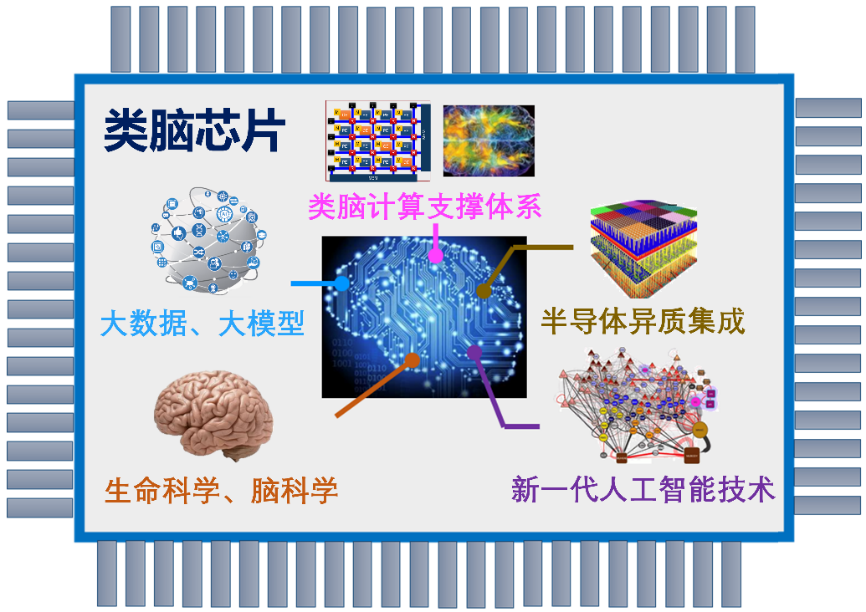
\includegraphics[width=0.8\linewidth]{5.png}
    \caption{类脑芯片宏观架构}
\end{figure}
\subsection{Loihi (Intel)}
\subsubsection{架构特点}
\begin{itemize}
    \item 异步事件驱动: Loihi 采用全异步事件驱动架构,神经元和突触的活动都是基于事件触发的,最大程度地降低了功耗。
    \item 分布式神经元核心: 芯片包含 128 个神经元核心,每个核心包含 1024 个脉冲神经元,共计 131,072 个神经元。
    \item 可编程神经元模型: 支持多种神经元模型,包括 LIF, Integrate-and-Fire 等。
    \item 片上学习: 硬件实现 STDP 等脉冲学习规则,支持片上学习。
    \item NoC 互连: 采用片上网络 (Network-on-Chip, NoC) 实现神经元核心之间的互连,支持大规模 SNN 模型。
\end{itemize}
\subsubsection{性能}
\begin{itemize}
    \item 神经元容量: 131,072 神经元
    \item 突触容量: 1.3 亿突触
    \item 功耗: ~150mW (运行典型 SNN 应用时)
    \item 应用: 模式识别、路径规划、优化问题等
\end{itemize}
\subsection{TrueNorth (IBM)}
\subsubsection{架构特点}
\begin{itemize}
    \item 大规模并行: TrueNorth 芯片包含 4096 个神经突触核心,每个核心包含 256 个神经元,共计 100 万个神经元。
    \item 二进制脉冲: 神经元之间传递二进制脉冲 (0 或 1)。
    \item 确定性神经元模型: 采用简化的确定性神经元模型。
    \item 片上学习: 支持有限的片上学习能力。
    \item 2D Mesh 互连: 采用二维网格 (2D Mesh) 结构实现神经突触核心之间的互连。
\end{itemize}
\subsubsection{性能}
\begin{itemize}
    \item 神经元容量: 100 万神经元
    \item 突触容量: 2.56 亿突触
    \item 功耗: ~70mW (运行实时生物神经网络仿真时)
    \item 应用: 图像识别、视频处理、模式分类等
\end{itemize}
\subsection{SpiNNaker (Manchester University)}
\subsubsection{架构特点}
\begin{itemize}
    \item 通用数字处理器: SpiNNaker 基于 ARM 处理器内核构建,每个芯片包含 18 个 ARM 内核,可灵活地配置和运行各种 SNN 模型。
    \item 软件可编程性强: 用户可以使用 SpiNNaker 软件工具链灵活地定义神经元模型、网络结构和学习规则。
    \item 大规模互连: 采用定制的互连网络实现芯片之间的互连,可构建包含数百万神经元的大规模 SNN 系统。
\end{itemize}
\subsubsection{性能}
\begin{itemize}
    \item 神经元容量: 单芯片可模拟数千神经元,多芯片系统可扩展至数百万神经元
    \item 突触容量: 单芯片可支持数百万突触,多芯片系统可扩展至数十亿突触
    \item 功耗: 单芯片 ~1W
    \item 应用: 大规模生物神经网络仿真、神经科学研究、SNN 算法验证等
\end{itemize}
\subsection{Tianjic (清华大学)}
\subsubsection{架构特点}
\begin{itemize}
    \item 混合架构: Tianjic 芯片采用混合架构,融合了类脑计算和传统机器学习的特点,既支持 SNN,也支持 ANN。
    \item 异构计算核心: 包含多种类型的计算核心,例如神经形态核心 (NorCore) 和机器学习核心 (MLCore),分别用于加速 SNN 和 ANN 运算。
    \item 片上总线互连: 采用片上总线 (Bus) 实现不同类型计算核心之间的互连。
\end{itemize}
\subsubsection{性能}
\begin{itemize}
    \item 神经元容量: 156 万神经元
    \item 突触容量: 100 亿突触
    \item 功耗: ~5W
    \item 应用: 自动驾驶、机器人、智能硬件等
\end{itemize}
各类脑芯片的性能对比,如表\ref{table-3}
% Please add the following required packages to your document preamble:
% \usepackage{booktabs}
\begin{table}[!h]
\caption{类脑芯片的性能对比} \label{table-3} \vspace{2mm}
\begin{tabularx}{\textwidth}{llllll}
\toprule
\multicolumn{1}{c}{\textbf{芯片}} & \multicolumn{1}{c}{\textbf{神经元容量}} & \multicolumn{1}{c}{\textbf{突触容量}} & \multicolumn{1}{c}{\textbf{功耗}} & \multicolumn{1}{c}{\textbf{架构特点}}                          & \multicolumn{1}{c}{\textbf{应用场景}}                         \\ \midrule
\textbf{Loihi}                  & 13 万                               & 1.3 亿                             & $\sim$150mW                     & \begin{tabular}[c]{@{}l@{}}异步事件驱动,\\ 片上学习\end{tabular}     & \begin{tabular}[c]{@{}l@{}}模式识别、\\ 优化问题等\end{tabular}     \\
\textbf{TrueNorth}              & 100 万                              & 2.56 亿                            & $\sim$70mW                      & \begin{tabular}[c]{@{}l@{}}大规模并行,\\ 二进制脉冲\end{tabular}     & \begin{tabular}[c]{@{}l@{}}图像识别、\\ 视频处理等\end{tabular}     \\
\textbf{SpiNNaker}              & 数百万                                & 数十亿                               & $\sim$1W                        & \begin{tabular}[c]{@{}l@{}}通用数字处理器,\\ 软件可编程性强\end{tabular} & \begin{tabular}[c]{@{}l@{}}生物网络仿真、\\ 算法验证等\end{tabular} \\
\textbf{Tianjic}                & 156 万                              & 100 亿                             & $\sim$5W                        & \begin{tabular}[c]{@{}l@{}}混合架构,\\ 异构计算核心\end{tabular}     & \begin{tabular}[c]{@{}l@{}}自动驾驶、\\ 机器人等\end{tabular}      \\ \bottomrule
\end{tabularx}
\end{table}
\subsection{总结}
各类脑芯片在架构设计和性能指标上各有侧重,例如 Loihi 和 TrueNorth 侧重于低功耗和事件驱动特性,SpiNNaker 侧重于灵活性和可扩展性,Tianjic 则侧重于混合计算能力。用户需要根据具体的应用需求选择合适的类脑芯片。未来类脑芯片的发展趋势将朝着更大规模、更高性能、更低功耗、更灵活可编程的方向发展。

\section{应用场景}
类脑芯片和脉冲神经网络 (SNN) 由于其独特的优势,在多个领域展现出广阔的应用前景\cite{ref9,ref10}:
\begin{figure}[htbp]
    \centering
    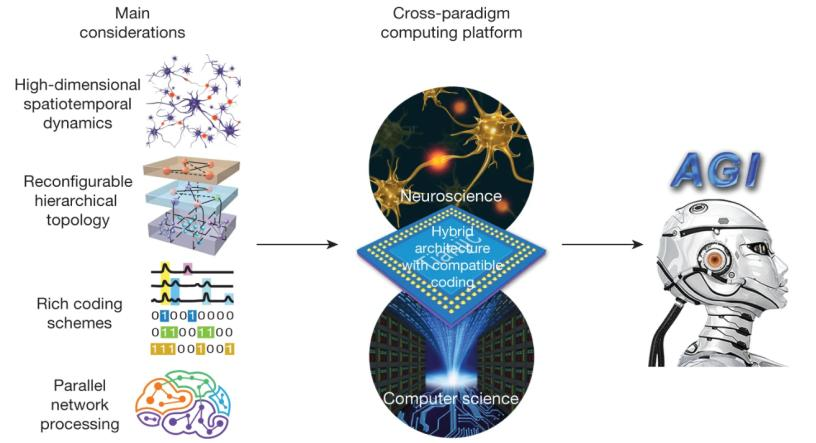
\includegraphics[width=\linewidth]{6.jpeg}
    \caption{类脑芯片的应用场景}
\end{figure}
\begin{itemize}
    \item \textbf{低功耗边缘计算:} SNN 的事件驱动和稀疏计算特性,使得类脑芯片在功耗方面具有显著优势,非常适合于低功耗边缘计算设备,例如:
    \begin{itemize}
        \item \textbf{移动设备:} 智能手机、可穿戴设备等,用于实现本地化的 AI 功能,例如图像识别、语音识别、自然语言处理等,降低设备功耗,延长电池续航时间。
        \item \textbf{物联网设备:} 智能传感器、智能家居设备等,用于实现边缘数据处理和分析,降低数据传输量,提高响应速度和隐私安全性。
        \item \textbf{自动驾驶:} 车载计算平台,用于实时处理传感器数据 (如摄像头、激光雷达等),实现环境感知、路径规划和决策控制,提高自动驾驶系统的安全性和可靠性。
    \end{itemize}
    \item \textbf{时序数据处理:} SNN 能够自然地处理时序信息,例如脉冲发放的时间、频率和模式等,这使得类脑芯片在时序数据处理领域具有优势,例如:
    \begin{itemize}
        \item \textbf{语音识别:} 处理语音信号的时序特征,提高语音识别的准确率和鲁棒性,尤其是在噪声环境和低功耗场景下。
        \item \textbf{视频分析:} 处理视频序列的时序信息,进行动作识别、场景理解、事件检测等,应用于智能监控、视频搜索、行为分析等领域。
        \item \textbf{金融时间序列预测:} 分析股票价格、交易量等金融时间序列数据,进行趋势预测和风险评估。
        \item \textbf{生物信号处理:} 处理脑电信号 (EEG)、心电信号 (ECG) 等生物信号,进行疾病诊断、健康监测、脑机接口等应用。
    \end{itemize}
    \item \textbf{神经科学研究:} 类脑芯片为神经科学研究提供了强大的工具,可以用于:
    \begin{itemize}
        \item \textbf{大规模生物神经网络仿真:} 模拟大规模生物神经网络的结构和功能,研究大脑的工作原理、信息处理机制、学习和记忆机制等。
        \item \textbf{神经疾病建模与治疗:} 建立神经疾病 (如帕金森病、阿尔茨海默病等) 的计算模型,研究疾病的发生机制、发展过程和潜在的治疗方法。
        \item \textbf{脑机接口:} 构建新型脑机接口系统,实现人脑与外部设备的直接信息交互,用于运动功能康复、意识解码、增强智能等。
    \end{itemize}
    \item \textbf{新型计算范式探索:} 类脑计算作为一种全新的计算范式,为探索新型计算模型和算法提供了平台,例如:
    \begin{itemize}
        \item \textbf{类脑学习算法研究:} 在类脑芯片上实现和验证各种生物 plausibility 较高的学习算法 (如 STDP),探索更高效、更鲁棒的学习机制。
        \item \textbf{新型人工智能应用:} 探索基于类脑计算的新型人工智能应用,例如类脑机器人、类脑智能体等,实现更接近人脑智能水平的 AI 系统。
    \end{itemize}
\end{itemize}
类脑芯片和 SNN 在低功耗、时序数据处理、生物合理性等方面具有独特的优势,使其在边缘计算、时序数据处理、神经科学研究和新型计算范式探索等领域展现出广阔的应用前景。随着类脑芯片技术的不断发展和成熟,相信未来将在更多领域看到类脑计算的身影。

\section{报告总结}
类脑芯片和脉冲神经网络 (SNN) 代表了人工智能领域的一个重要发展方向。它们从生物神经系统中汲取灵感,旨在突破传统计算架构的瓶颈,构建更高效、更低功耗、更智能的计算系统\cite{ref11}。

\paragraph{主要优势}

\begin{itemize}
    \item \textbf{低功耗:} 事件驱动和脉冲稀疏性使得 SNN 和类脑芯片在功耗方面具有显著优势,尤其适合于边缘计算和移动设备等应用。
    \item \textbf{时序信息处理能力:} SNN 能够自然地处理时序信息,在语音、视频、生物信号等时序数据处理领域具有优势。
    \item \textbf{生物合理性:} SNN 更接近生物神经网络的工作方式,为神经科学研究提供了有力的工具,并有望启发更通用的人工智能。
    \item \textbf{硬件友好性:} SNN 与神经形态硬件天然契合,类脑芯片为 SNN 的高效运行和应用提供了理想的硬件平台。
\end{itemize}

\paragraph{面临的挑战}

\begin{itemize}
    \item \textbf{学习算法的复杂性:} SNN 的学习算法相对 ANN 更加复杂,训练 SNN 模型仍然是一个挑战。
    \item \textbf{模型优化的难度:} SNN 模型参数众多,优化难度较大,需要更有效的模型优化方法。
    \item \textbf{硬件实现的挑战:} 大规模、高性能 SNN 硬件的实现仍然面临技术挑战。
    \item \textbf{应用生态的完善:} SNN 的应用生态尚不完善,需要开发更多的 SNN 应用案例,拓展应用领域。
\end{itemize}

\paragraph{未来展望}

尽管面临一些挑战,但类脑芯片和 SNN 的发展前景依然广阔。随着技术的不断进步,相信未来类脑芯片将在以下方面取得重要突破:

\begin{itemize}
    \item \textbf{更大规模和更高性能的芯片:} 随着集成电路技术的进步,类脑芯片的神经元容量、突触容量和计算性能将持续提升,能够支持更大规模、更复杂的 SNN 模型。
    \item \textbf{更低功耗的设计:} 新型材料、器件和电路设计技术的应用,将进一步降低类脑芯片的功耗,使其更适合于各种低功耗应用场景。
    \item \textbf{更灵活可编程的架构:} 未来的类脑芯片将更加注重可编程性,支持用户灵活地配置神经元模型、网络结构和学习规则,满足不同应用的需求。
    \item \textbf{更完善的软件工具链:} 为了降低 SNN 的开发门槛,需要开发更完善的 SNN 软件工具链,包括模型构建、训练、仿真、部署等工具。
    \item \textbf{更广泛的应用领域:} 随着技术的成熟和应用案例的积累,类脑芯片和 SNN 将在更多领域得到应用,例如边缘智能、时序数据处理、神经科学研究、新型计算范式等。
\end{itemize}

总而言之,类脑芯片和 SNN 作为新兴技术,正处于快速发展阶段。虽然距离真正模拟人脑智能还有很长的路要走,但它们已经展现出巨大的潜力,有望为人工智能的未来发展带来革命性的变革。

\begin{thebibliography}{99}  
    \bibitem{ref1}郑南宁,任鹏举,陈霸东,等.类脑(受脑启发的)计算的问题与视觉认知[C]//中国科学技术协会,吉林省人民政府.第十九届中国科协年会——分5“智能制造引领东北工业基地振兴”交流研讨会论文集.西安交通大学人工智能与机器人研究所;,2017:3. 
    \bibitem{ref2}B. Yin, F. Corradi, and S. M. Bohte, “Effective and Efficient Computation with Multiple-timescale Spiking Recurrent Neural Networks,” Data Archiving and Networked Services (DANS), Jul. 2020, doi: https://doi.org/10.1145/3407197.3407225.
    \bibitem{ref3}B. Yin, F. Corradi, and S. M. Bohté, “Accurate and efficient time-domain classification with adaptive spiking recurrent neural networks,” Nature Machine Intelligence, vol. 3, no. 10, pp. 905–913, Oct. 2021, doi: https://doi.org/10.1038/s42256-021-00397-w.
    \bibitem{ref4}L. Deng et al., “Rethinking the performance comparison between SNNS and ANNS,” Neural Networks, vol. 121, pp. 294–307, Jan. 2020, doi: https://doi.org/10.1016/j.neunet.2019.09.005.
    \bibitem{ref5}F. Liu, W. Zhao, Y. Chen, Z. Wang, and L. Jiang, “SpikeConverter: An Efficient Conversion Framework Zipping the Gap between Artificial Neural Networks and Spiking Neural Networks,” Proceedings of the AAAI Conference on Artificial Intelligence, vol. 36, no. 2, pp. 1692–1701, Jun. 2022, doi: https://doi.org/10.1609/aaai.v36i2.20061.
    \bibitem{ref6}Maass W Networks of spiking neurons: the third generation of neural network models. Neural Netw. 1997;10(9):1659–1671. doi: 10.1016/S0893-6080(97)00011-7.
    \bibitem{ref7}Hodgkin A L, Huxley A F A quantitative description of membrane current and its application to conduction and excitation in nerve. J Physiol. 1952;117(4):500–544. doi: 10.1113/jphysiol.1952.sp004764.
    \bibitem{ref8}Abbott L F Lapicque's introduction of the integrate-and-fire model neuron. Brain Res Bull. 2000;50(5/6):303–304. doi: 10.1016/s0361-9230(99)00161-6.
    \bibitem{ref9}“类脑芯片-上海交通大学类脑智能应用与技术中心,” Sjtu.edu.cn, 2025. https://bat.sjtu.edu.cn/zh/satellite-navigation/
    \bibitem{ref10}“类脑芯片:人造电子大脑,” Dec. 20, 2023. https://36kr.com/p/2568941971824520
    \bibitem{ref11}“一文梳理类脑计算的前世今生 | 中科院自动化所研究员李国齐,” Shisu.edu.cn, 2022. https://aidc.shisu.edu.cn/66/2f/c11041a157231/page.htm
\end{thebibliography}


\end{document}
